\documentclass[11pt, a4paper]{article}

\usepackage[T2A]{fontenc}		%cyrillic output
\usepackage[utf8]{inputenc}		%cyrillic output
\usepackage[english, russian]{babel}	%word wrap
\usepackage{amssymb, amsfonts, amsmath}	%math symbols
\usepackage{mathtext}			%text in formulas
\usepackage{geometry}			%paper format attributes
\usepackage{fancyhdr}			%header
\usepackage{graphicx}			%input pictures
\usepackage{tikz}				%draw pictures
\usetikzlibrary{patterns}		%draw pictures: fill
\usepackage{enumitem}			%enumarate parameters

\geometry{left=1cm, right=1cm, top=2cm, bottom=1cm, headheight=15pt}
\setlist[enumerate]{leftmargin=*}	%remove enumarate indenttion
\sloppy							%correct overfull

\newcommand{\head}[4]
{
	\pagestyle{fancy}
	\fancyhf{}
	\chead{#3, #4}

	\begin{center}
	\begin{large}
	#1 \\
	\textit{#2}\\
	\end{large}
	\end{center}

}

\begin{document}

\head{Открытая студенческая олимпиада по математике \\ Казахстанского филиала МГУ}{10 декабря 2014}{Казахстанский филиал МГУ имени М. В. Ломоносова}{г. Астана}

\begin{enumerate}
\item Ответ: $f(x) = x - \frac{3}{2}$. Рассмотрим функцию 
$$g(x) = f(x) - \left(x - \frac{3}{2}\right).$$
Она непрерывна и удовлетворяет соотношению 
$$g(2x+1) = \frac{1}{3} g(x),$$ 
для любого $x \in \mathbb{R}$. После замены $t = 2x+1$:
$$g(t) = \frac{1}{3} g\left( \frac{t-1}{2} \right).$$
Отсюда $g(-1) = 0$. Далее, для каждого $y \in \mathbb{R}$ рассмотрим последовательность, заданную рекуррентным способом: 
$$\begin{cases}
y_1 = y, \\
y_{n+1} = \frac{y_n-1}{2}.
\end{cases}$$
Тогда $\lim_{n \to \infty} {y_n} = -1$ и $g(y_n) = \frac{1}{3} g(y_{n+1})$ для всех $y \in \mathbb{R}$. 
Значит,
$$g(y) = \frac{1}{3^n} g(y_{n}).$$
В силу непрерывности имеем $g(y) = 0$.  

\item Ответ: $-\frac{\pi^2}{18}$.

Во-первых:
$$
\int\limits_{0}^{1} \frac{\ln(1-u)}{u} \,du = 
\{ u = v^2 \} = 
2 \int\limits_{0}^{1} \frac{\ln(1-v^2)}{v} \,dv = $$
$$=2 \left( 
\int\limits_{0}^{1} \frac{\ln(1-v)}{v} \,dv 
+
\int\limits_{0}^{1} \frac{\ln(1+v)}{v} \,dv
\right),
$$
то есть
$$
\int\limits_{0}^{1} \frac{\ln(1-u)}{u} \,du = 
-2 \int\limits_{0}^{1} \frac{\ln(1+v)}{v} \,dv .
$$

Во-вторых:
$$
\int\limits_{0}^{1} \frac{\ln(1-u)}{u} \,du = 
\{ z = v^3 \} = 
3 \int\limits_{0}^{1} \frac{\ln(1-z^3)}{z} \,dz$$


\item Ответ: нет. Для некоторого $N \in \mathbb{N}$:
$$\sum_{n=1}^{\infty} \frac{\varepsilon_n}{n!} =
\sum_{n=1}^{N} \frac{\varepsilon_n}{n!} +
\sum_{n=N+1}^{\infty} \frac{\varepsilon_n}{n!} =
\frac{H}{N!} + r_N,$$
где $H \in \mathbb{Z}$ и 
$$|r_N| \leqslant \sum_{n=N+1}^{\infty} \frac{1}{n!} = \frac{1}{(N+1)!} \left( 1 + \frac{1}{N+2} + ... \right) < $$
$$ < \frac{3}{2} \cdot \frac{1}{(N+1)!} < \frac{1}{N!}.$$
При этом $r_N \neq 0$, так как $r_{N} = \frac{1}{(N+1)!} \varepsilon_{N+1} + r_{N+1}$ и $|r_{N+1}| < \frac{1}{(N+1)!}$.

\item (Абдикалыков А.К.) Пусть $f(\lambda) = |B-\lambda I|$ --- характеристический многочлен матрицы $B$. Заметим, что требуется доказать то, что $f(1)\ne 0$; другими словами, то, что число 1 не является собственным значением матрицы $B$. А поскольку из $AB=A+2014B$ следует $(A-2014I)(B-I)=2014I$, то матрица $B-I$ обязана быть невырожденной.

\item Ответ: при четном $n$ выиграет начинающий, а при нечетном --- его соперник. Легко заметить, что если текущее число нечетное, то игрок изменит число на четное; а если четное, то игрок всегда может уменьшить число на 1.

\item Пусть $x$ таково, что $x^3-x-1=0$. Но тогда
$$
x^5-x^4-1=(x^2-x+1)(x^3-x-1)=0.$$

\item Ответ: $\frac{\pi}{4}$. Из тождества 
$$F_{n-1}F_{n+1}=F^2_n+(-1)^n$$
можно получить соотношение $$\mathrm{arcctg}\,{F_{2n+1}}=\mathrm{arcctg}\,{F_{2n}}-\mathrm{arcctg}\,{F_{2n+2}}.$$
Искомая сумма, таким образом, будет равна $$\mathrm{arcctg}\,{F_2}=\pi/4.$$

\item Все перестановки, обратные сами себе, можно представить в виде композиции непересекающихся циклов длины 2. Число перестановок $\alpha$ порядка $n+1$ таких, что $\alpha=\alpha^{-1}$ и $\alpha_{n+1}=n+1$, очевидно, равно $a_n$; число же перестановок $\alpha$ порядка $n+1$ таких, что $\alpha=\alpha^{-1}$ и $\alpha_{n+1}=k\not=n+1$ для некоторого фиксированного $k$, равно $a_{n-1}$. Общее число инволюций порядка $n+1$ равно $a_{n+1} = a_n + na_{n-1}$.

\item (Баев А.Ж.) Ответ: 24. Пусть столбцов не меньше, чем строк. Если столбцов не менее 5, то строк менее 5. Доказательство от противного (в первой строке как минимум 3 клетки одного цвета, значит, в остальных строках обязательно найдется прямоугольник с клетками противоположного цвета). Если строк 3 или 4, то столбцов менее 7 (доказательство аналогично предыдущему). 

Так как столбцов не более 6, строк не более 4, то ответ 24. Пример:
\begin{center}
\begin{tabular}{|c|c|c|c|c|c|}
\hline
A & A & A & B & B & B \\
\hline
A & B & B & B & A & A \\
\hline
B & A & B & A & B & A \\
\hline
B & B & A & A & A & B \\
\hline
\end{tabular}
\end{center}

\item Обозначим: $KLM$ --- исходный треугольник, $A$, $B$, $C$ --- точки касания параболы и прямых $MK$, $KL$, $LM$. $A_2$, $B_2$, $C_2$ --- проекции $A$, $B$, $C$ на директрису. $F$ --- фокус параболы. $A_1$, $B_1$, $C_1$ --- середины $A_2F$, $B_2F$, $C_2F$.

\begin{center}
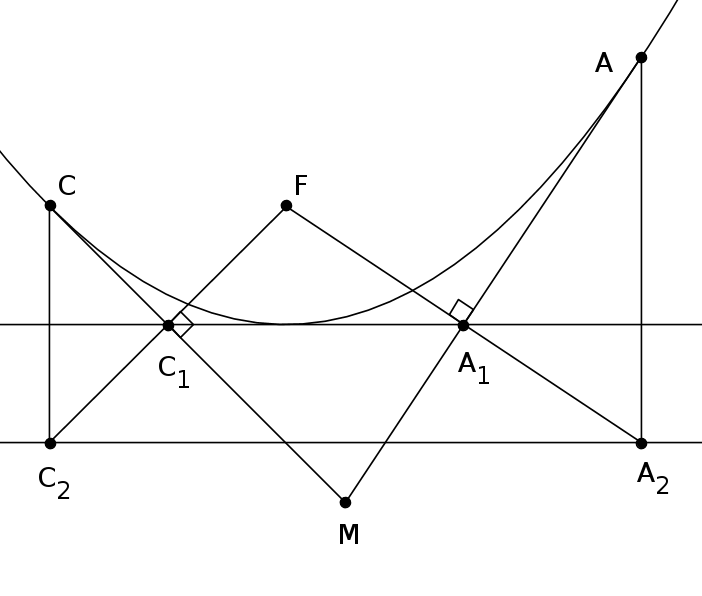
\includegraphics{pictures/2014-2015-10-1}
\end{center}

Свойство 1. Прямая, содержащая $A_1B_1C_1$, является касательной к параболе и параллельна директрисе. Данный факт легко получить из оптического свойства параболы и определения параболы (треугольник $FAA_2$ --- равнобедренный).

Свойство 2. Треугольники $FA_1K$ и $FC_1L$ подобны. Данный факт получается из вписанных четырехугольников $FKA_1B_1$ и $FB_1LC_1$.

Обозначим: $L_1$ --- основание высоты из $L$ на $KM$, $K_1$ --- основание высоты из $K$ на $LM$. $P$ и $Q$ --- точки пересечения $LL_1$ и $KK_1$ с $A_1C_1$.

\begin{center}
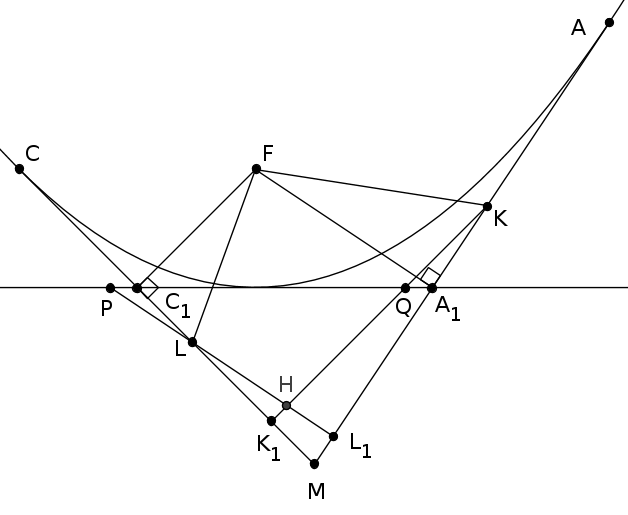
\includegraphics[width=8cm]{pictures/2014-2015-10-2}
\end{center}

Свойство 3. $A_1Q = PC_1$. По соответствующим теоремам синусов для треугольников $PC_1L$, $KA_1Q$ и $C_1FA_1$ можно получить, что 
$$ \frac{PC_1}{A_1Q} = \frac{C_1L}{A_1K} \cdot \frac{\sin Q}{\sin P} = \frac{C_1L}{A_1K} \cdot \frac{\sin C_1}{\sin A_1} = \frac{C_1L}{A_1K} \cdot \frac{A_1F}{C_1F} = 1$$
Последнее верно из свойства 2.

Свойство 3. $H$ лежит на директрисе. Для этого достаточно заметить, что треугольники $PHQ$ и $A_1FC_1$ равны. Значит, расстояние от $H$ и $F$ до прямой $A_1C_1$ одинаково.


\end{enumerate}

\end{document} 
